\documentclass[12pt]{article}
\usepackage[margin=1in]{geometry}
\usepackage{graphicx}
\usepackage{hyperref}
\usepackage{enumitem}
\usepackage{ulem}
\usepackage{setspace}
\usepackage[usenames,dvipsnames]{xcolor}
\setlength\parindent{0pt}

\begin{document}

\title{Lab 1: Introduction to Quarto}
\author{Qian Wu}
\date{2025 Fall Session 2}

\maketitle
\begin{center}
   click \href{https://qianwu-dku.github.io/STAT101/Lab1/lab1_instruction.pdf}{here} for latest version   
\end{center}
\section{What is Quarto?}
Quarto is a document container that allows you to mix code, output, and text to produce reproducible results and auto-generate high quality document. 

\section{Install Quarto}
To install Quarto, please enter the following line of code in the Terminal window (not the Console window):    
\begin{verbatim}
    quarto install tinytex
\end{verbatim}
\begin{center}
    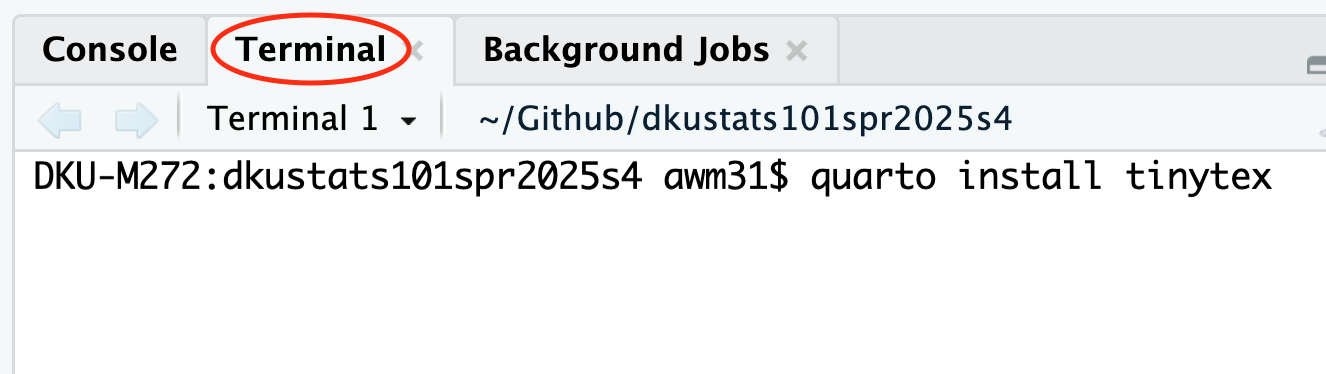
\includegraphics[scale=0.3]{Terminal.png}
\end{center}


\section{Practicing with Quarto}
To complete this lab, please do a simple investigation into the distribution of \textbf{mpg} (miles per gallon) and \textbf{wt} (weight) from the \textbf{mtcars} built-in dataset.
\begin{enumerate}
    \item Select File $\rightarrow$ New File $\rightarrow$ Quarto Document. 
    \item Create YAML header.
    \item Insert an R code block and then make a histogram of \textbf{mpg}.
    \item Describe features of the mpg distribution (center, spread).
    \item Repeat for the variable \textbf{wt}.
    \item Add appropriate headers for each section and make sure you can navigate between them.
    \item Write a brief conclusion of your investigation.
\end{enumerate}
Feeling overwhelmed? Turn to next page for step-by-step instructions!

\subsection{Two Views to Edit Document}
RStudio has two views for editing your document, Source and Visual. 
\begin{center}
   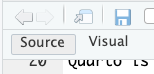
\includegraphics[scale=.8]{editmode.png} 
\end{center}
Most people find it easier to edit using the Visual mode. Switch back and forth between the
two views to check the differences.

\subsection{Create YAML Header}
At the top of your document, there is a metadata block that controls the document's properties and appearance. This is the YAML header.

\begin{center}
   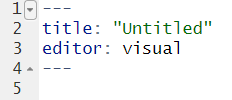
\includegraphics[scale=.8]{yamlblock.png} 
\end{center}

You CANNOT put R code in this section and it must always be at the top of your document.
For common YAML fields, check \href{https://quarto.org/docs/reference/formats/html.html}{here}. 

\textcolor{blue}{Please add a subtitle and an abstract to your YAML header.}


\subsection{Insert R Code Block}
To write R code, you need to add a code block with the ``Insert a New Code Chunk" button.
\begin{center}
    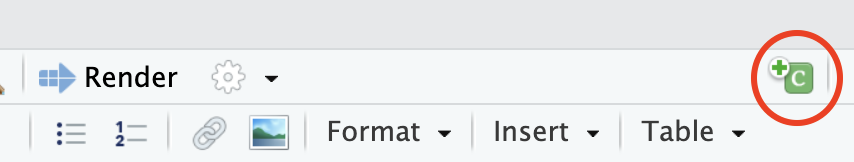
\includegraphics[scale=.8]{Insert code block.png}
\end{center}

\subsubsection{Setup block}
We often begin the R code with the setup block. In the setup block, you will set working directory, clean objectives, and library (load) all packages needed to run the code.\footnote{Note: do not put install packages commands. You only need to install
packages once.} A good setup block looks like this:
\begin{center}
    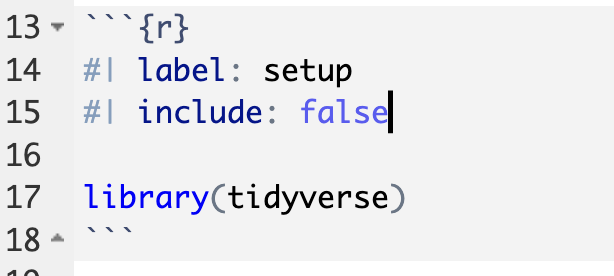
\includegraphics[scale=.7]{setupblock.png}
\end{center}
\textcolor{blue}{Please add a setup block to load the \textbf{tidyverse} library.} 


\subsubsection{Other blocks}
You might notice that, the setup bock contains ``\verb!#|!" symbols. In Quarto, the ``\verb!#|!" prefix in a code block is used for YAML option syntax within code cells. It allows you to specify cell-specific options directly in the code chunk. Each code block header starts with
\begin{verbatim}
    #| <option>: <value>
\end{verbatim}
For example, here is a simple code block to produce a histogram with ggplot function.
\begin{center}
    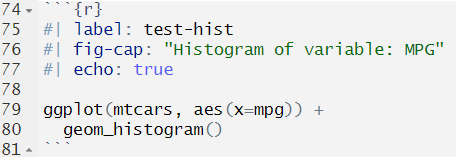
\includegraphics[scale=.8]{histsample.png}
\end{center}
What do the code block headers (line 75-77) do? 
\begin{itemize}
    \item ``\verb!#| label: test-hist!" labels this code block, indicating we are creating a test histogram. \footnote{It's a good habit to label each code block so it is easy to move around your document and recall what each block does. }
    \item ``\verb!#| fig-cap: "Histogram of variable: MPG"!" assigns the caption ``Histogram of variable: MPG" to the output histogram. 
    \item ``\verb!#| echo: true!" specifies both the R code and the output histogram (with caption) should appear in the rendered PDF.
\end{itemize}
The remaining lines (line 79-80) use ggplot function to draw a histogram for the variable \textbf{mpg} in the dataset \textbf{mtcars}.

\textcolor{blue}{Please create two code blocks, one that produces a histogram of the variable \textbf{mpg} and the other that finds the mean and the standard deviation of \textbf{mpg} (you can use the following code example below). Label these two blocks and your setup block.}
\begin{verbatim}
    mtcars %>%
      summarise(mean_mpg = mean(mpg), sd_mpg = sd(mpg))
\end{verbatim}


\subsection{Execute Code}
There are two ways to execute (run) your code.
\begin{itemize}
    \item Execute entire script: The Render button renders your document from the very first block, going all the way to the end (unless there is an error, in which case it will stop).
    \begin{center}
        
\includegraphics[scale=.8]{render.png}
    \end{center}
    \item Execute each block: The green triangle on the right top corner exceutes only the code in that block. This can be useful to quickly check if your code works. However, it can be dangerous because (1) it can call back the objectives you have deleted the code for; (2) the preview window can display unreliable formats.
    \begin{center}
        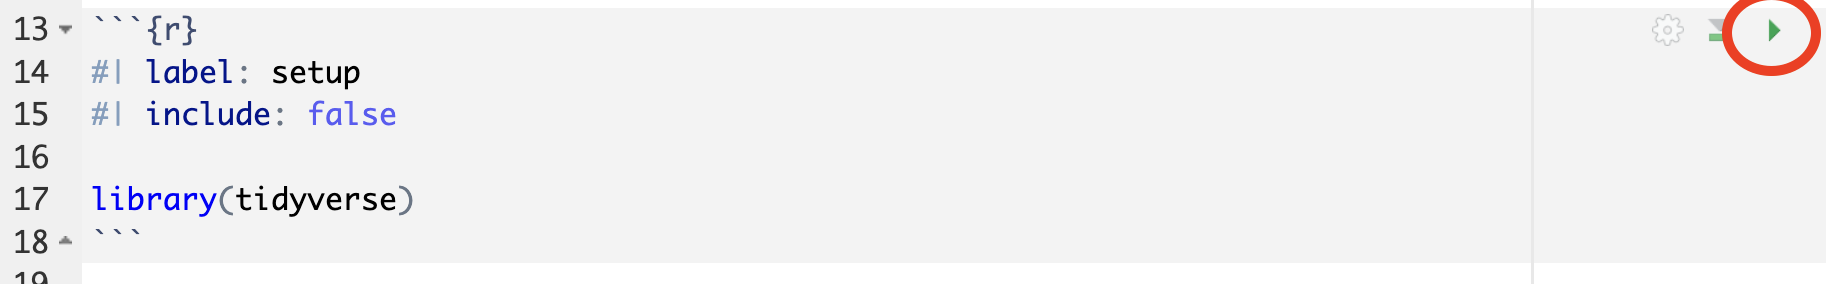
\includegraphics[scale=.5]{greentriangle.png}
    \end{center}
    I consider it best practice to use the Render button regularly to make sure your document will work at submission time and display the way you prefer. 
\end{itemize}
\textcolor{blue}{Please click Render button and verify your document will produce the desired outcome.}

\subsection{Label Graphs and Tables}
Sometimes, we want to auto-number and cross-reference graphs and tables throughout a document.\footnote{See \href{https://quarto.org/docs/authoring/figures.html\#cross-references}{here} and \href{https://quarto.org/docs/authoring/tables.html\#cross-references}{here} for instructions on graphs and tables, respectively.} Quarto allows us to do these in a systematic way. For code blocks with figures, we can label figures by adding a block header:
\begin{verbatim}
    #| label: fig-<your choice of label>
\end{verbatim}
For example, ``\verb!#| label: fig-mtcarsmpghist!" can be a good label for the histogram of \textbf{mpg} in the dataset \textbf{mtcars}.

\textcolor{blue}{Replace the} ``\verb!#| label: test-hist!" \textcolor{blue}{header with} ``\verb!#| label: fig-<your choice of label>! \textcolor{blue}{to label your histogram.} 

When there are multiple graphs, you can assign different captions to them by adding a block header:
\begin{verbatim}
    #| fig-subcap: 
    #|   - "<caption for subgraph 1>"
    #|   - "<caption for subgraph 2>"
\end{verbatim}
\textcolor{blue}{Following \href{https://quarto.org/docs/authoring/figures.html\#subcaptions}{this page}, in the test-hist block, add a second histogram of \textbf{mtcars\$mpg} but change the binwidth. Create subcaptions for the two plots.}


\subsection{Repeat for Variable wt}
\textcolor{blue}{Now repeat the operations above for the variable \textbf{wt}: draw histogram and calculate mean and standard deviation. Write a few sentences interpreting your results.}

\subsubsection{Navigate document}
To make your document navigable (auto-generate a content), you need to specify headings for your document sections. We use ``\verb!#!" for sections, ``\verb!##!" for subsections, and so on so forth.
    \begin{center}
        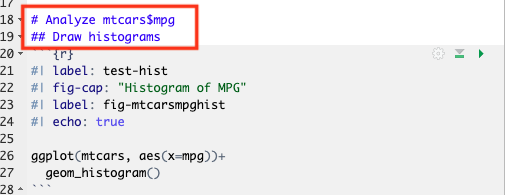
\includegraphics[scale=.7]{headings.png}
    \end{center}

You can navigate your document in two ways.
\begin{itemize}
    \item Outline window on the top right corner.
    \begin{center}
        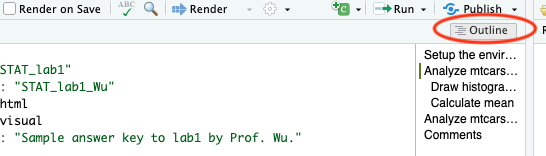
\includegraphics[scale=.7]{outline.png}
    \end{center}
    \item Menu list on the bottom left corner. 
        \begin{center}
        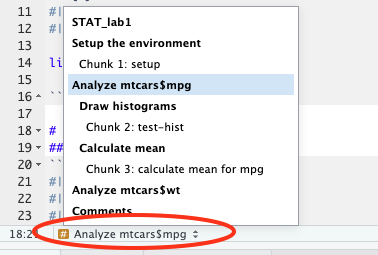
\includegraphics[scale=.7]{menu.png}
    \end{center}
\end{itemize}
\section{Finish up}
Once you finish, please show me your result and then you can proceed to \href{https://quarto.org/docs/get-started/computations/rstudio.html}{this website} for a computations tutorial. Please try to modify your document according to the exercises on the
tutorial webpage until the end of class.
\end{document}
